\documentclass[dvisvgm,tikz,border=4pt]{standalone}
\usepackage{amsmath,amssymb}

\usetikzlibrary{arrows.meta,positioning,automata,shapes,shapes.misc,calc,decorations.pathmorphing,decorations.markings,angles,quotes,patterns,mindmap,matrix,knots,hobby,trees}
\tikzset{->-/.style={decoration={markings, mark=at position 0.5 with {\arrow{Stealth}}}, postaction={decorate}}}
\begin{document}
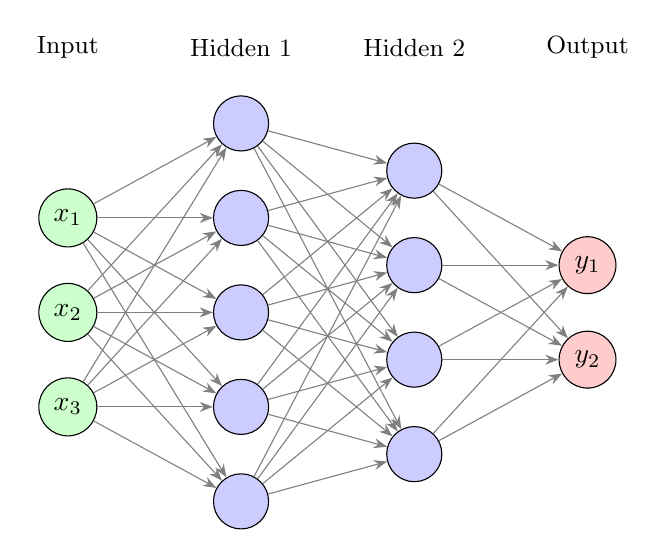
\begin{tikzpicture}[x=2.2cm, y=1.2cm, >=Stealth, n/.style={circle, draw, minimum size=7mm}]
\foreach \i in {1,...,3} \node[n, fill=green!20] (i\i) at (0,-\i) {$x_\i$};
\foreach \i in {1,...,5} \node[n, fill=blue!20] (h\i) at (1,-\i+1) {};
\foreach \i in {1,...,4} \node[n, fill=blue!20] (g\i) at (2,-\i+0.5) {};
\foreach \i in {1,...,2} \node[n, fill=red!20] (o\i) at (3,-\i-0.5) {$y_\i$};
\foreach \a in {1,...,3} \foreach \b in {1,...,5} \draw[->, gray] (i\a) -- (h\b);
\foreach \a in {1,...,5} \foreach \b in {1,...,4} \draw[->, gray] (h\a) -- (g\b);
\foreach \a in {1,...,4} \foreach \b in {1,...,2} \draw[->, gray] (g\a) -- (o\b);
\foreach \x/\l in {0/Input, 1/Hidden 1, 2/Hidden 2, 3/Output} \node[font=\small] at (\x,0.8) {\l};
\end{tikzpicture}
\end{document}
